\documentclass[conference]{IEEEtran}
\IEEEoverridecommandlockouts

\usepackage{cite}
\usepackage{amsmath,amssymb,amsfonts}
\usepackage{graphicx}
\usepackage{textcomp}
\usepackage{xcolor}
\usepackage{booktabs}
\usepackage{listings}
\usepackage{url}
\usepackage{multirow}

\lstset{
  basicstyle=\footnotesize\ttfamily,
  breaklines=true,
  frame=single,
  language=C,
  numbers=left,
  numberstyle=\tiny,
  xleftmargin=1.5em,
}

\begin{document}

\title{Lightweight Block Cipher Benchmarking for IoT and RFID:\\
SIMON 64/128 and GIFT-128 vs.\ AES-128}

\author{\IEEEauthorblockN{Narain Shriraam M S}
\IEEEauthorblockA{ECE Department\\
UC San Diego\\
A69041741}
\and
\IEEEauthorblockN{Karthik N R}
\IEEEauthorblockA{ECE Department\\
UC San Diego}
\and
\IEEEauthorblockN{Tushar Nasery}
\IEEEauthorblockA{ECE Department\\
UC San Diego}
}

\maketitle

\begin{abstract}
AES-128 dominates symmetric encryption in mainstream computing, but its
gate count and code footprint can be too large for passive RFID tags and
low-power sensor nodes.  In this paper we implement two lightweight block
ciphers in portable C: \textbf{SIMON~64/128}, a Feistel design from the
NSA SIMON family, and \textbf{GIFT-128/128}, an SPN cipher optimized for
small hardware area.  We wrap both in CBC and CTR modes, verify them
against published test vectors, and compare key-schedule latency,
cycles-per-byte throughput, and compiled code size to an \textbf{AES-128}
hardware-accelerated baseline.  On Apple Silicon (\texttt{gcc~-O2}),
SIMON runs at about 11~cpb in only 356~bytes of machine code; GIFT is
slower in software ($\approx$339~cpb) but the literature reports it at
roughly 1300~GE in silicon, well below AES.  We also wrote pure CUDA
kernels and measured CTR-mode speedups of $420\times$ for SIMON and
$388\times$ for GIFT on a Tesla~T4 GPU.  These numbers show that
lightweight ciphers are a practical alternative to AES when dedicated
hardware acceleration is not available, and that the choice between
Feistel and SPN has real consequences depending on whether the target is
software or silicon.
\end{abstract}

\begin{IEEEkeywords}
lightweight cryptography, SIMON, GIFT, block cipher, IoT, RFID, AES,
benchmark, CBC, CTR
\end{IEEEkeywords}

%===================================================================
\section{Introduction}
%===================================================================

As IoT devices and RFID tags become more widespread, there is growing
need for symmetric encryption that can work within very tight resource
budgets, sometimes as few as 1000--2000 gate equivalents (GE) with
limited RAM and code ROM~\cite{bogdanov2007present}.  AES-128 is the
standard choice for most systems, but even compact AES implementations
come in at 2400--3400~GE~\cite{feldhofer2004strong}, which is too large
for many passive RFID scenarios.

Several lightweight ciphers have been proposed to fill this gap.  We
focus on two that represent different design philosophies:

\begin{itemize}
\item \textbf{SIMON}~\cite{beaulieu2013simon} is a Feistel-network cipher
      family from the NSA.  It uses only circular shifts and bitwise
      AND/XOR, which keeps both code size and gate count small.
\item \textbf{GIFT}~\cite{banik2017gift} is an SPN (Substitution-Permutation
      Network) cipher that improves on PRESENT~\cite{bogdanov2007present}
      with better hardware efficiency and stronger security margins.
\end{itemize}

We implement \textbf{SIMON~64/128} (64-bit block, 128-bit key, 44~rounds)
and \textbf{GIFT-128/128} (128-bit block, 128-bit key, 40~rounds) in
portable C, add CBC and CTR mode wrappers, check correctness against
published test vectors, and measure performance relative to an AES-128
baseline.

%===================================================================
\section{Background}
%===================================================================

\subsection{AES-128 and Its Limitations}

AES operates on a $4\times4$ byte state matrix using a sequence of
SubBytes, ShiftRows, MixColumns, and AddRoundKey transformations over
10~rounds for a 128-bit key.  Modern desktop and server CPUs include
dedicated AES-NI instructions that reduce encryption to approximately
1--2~cycles/byte.  However, the MixColumns step requires either lookup
tables (consuming $>$1~KiB of ROM) or a Galois-field multiplier, both of
which are expensive in constrained hardware.  Feldhofer et
al.~\cite{feldhofer2004strong} demonstrated a compact AES implementation
for RFID at approximately 3,400~GE, but this is still above the budget of
many passive tags.

\subsection{The SIMON Family}

SIMON~$2n/mn$ uses a balanced Feistel network on two $n$-bit words with an
$mn$-bit key that gets expanded into $T$ round keys~\cite{beaulieu2013simon}.
The round function is
\[
f(x) = (x \lll 1\ \&\ x \lll 8) \oplus (x \lll 2)
\]
which needs just three circular left-shifts, one AND, and one XOR.  There
is no S-box, no multiplication, and no lookup table.  The key schedule generates round
keys using a linear recurrence with a $z$-sequence constant that depends on
$(n, m)$.

The SIMON family spans a wide range of parameters:

\begin{table}[htbp]
\caption{SIMON Family Parameters (Selected Variants)}
\label{tab:simonfamily}
\centering
\begin{tabular}{lcccl}
\toprule
\textbf{Variant} & $n$ & $m$ & \textbf{Rounds} & $z$\textbf{-seq} \\
\midrule
SIMON 32/64  & 16 & 4 & 32 & $z_0$ \\
SIMON 64/96  & 32 & 3 & 42 & $z_2$ \\
SIMON 64/128 & 32 & 4 & 44 & $z_3$ \\
SIMON 128/128 & 64 & 2 & 68 & $z_2$ \\
SIMON 128/256 & 64 & 4 & 72 & $z_4$ \\
\bottomrule
\end{tabular}
\end{table}

For our project we selected \textbf{SIMON~64/128}: $n=32$, $m=4$ key
words, $T=44$ rounds, $z$-sequence $z_3$.  This configuration provides a
128-bit security level with 64-bit blocks, suitable for message
authentication and short-message encryption in IoT.

Because of the Feistel structure, encryption and decryption use the same
round function.  Decryption just applies the round keys in reverse with
swapped halves, so we only need one copy of~$f$ in code.

\subsection{The GIFT Family}

GIFT-128~\cite{banik2017gift} is a 40-round SPN cipher that works on a
128-bit state stored as 32 four-bit nibbles.  It builds on PRESENT~\cite{bogdanov2007present}, with better security margins and lower
gate count.  Each round applies three operations:

\begin{enumerate}
\item \textbf{SubCells:} a 4-bit S-box $\{1,10,4,12,6,15,3,9,2,13,11,7,5,0,8,14\}$ independently to each nibble, providing non-linearity.
\item \textbf{PermBits:} a 128-bit bit permutation defined by a fixed table
      that achieves full diffusion across all four bit positions of every
      nibble after several rounds.
\item \textbf{AddRoundKey:} XOR of a 6-bit round constant (from a
      pre-computed LFSR sequence) and two 32-bit slices of the evolving key
      state into the $b_1$ and $b_2$ bit positions of each nibble.
\end{enumerate}

The 128-bit key state is updated after each round by a combination of
32-bit rotation of the entire key register and two 16-bit sub-word
rotations within the top two key words (by 12 and 2 positions
respectively).  Round constants are generated by a 6-bit LFSR and prevent
slide attacks.

The whole design was driven by gate count: the authors report about
1,300~GE for a round-unrolled version, below both AES and
PRESENT (1,570~GE).  GIFT also uses a 128-bit block, which avoids the
birthday-bound problems that come with 64-bit blocks.  One trade-off is
that GIFT's S-box is non-involutory, so decryption is slightly more
expensive, but this gives the cipher better algebraic properties.

\subsection{Modes of Operation}

Since both are block ciphers, they need a mode of operation to handle
messages longer than one block.  We implement two:

\begin{itemize}
\item \textbf{CBC (Cipher Block Chaining):} Each plaintext block is XORed
      with the previous ciphertext block before encryption.  We use PKCS\#7
      padding to handle messages whose length is not a multiple of the block
      size.
\item \textbf{CTR (Counter Mode):} A nonce-initialized counter is encrypted
      to produce a keystream that is XORed with plaintext.  CTR mode
      requires no padding and supports random access.
\end{itemize}

%===================================================================
\section{Design Choices}
%===================================================================

\subsection{Cipher Selection}

We had five ciphers to choose from (PRESENT-80, GIFT-128, SIMON-64,
SPECK-64, SKINNY-64).  We picked SIMON and GIFT because they cover both
major design families (Feistel and SPN) and have well-documented test
vectors and reference code.  We went with SIMON~64/128 instead of 64/96
because it gives a full 128-bit key and has a published test vector in
the specification appendix~\cite{beaulieu2013simon}.

\subsection{Data Representation}

\textbf{SIMON:} Block data is loaded/stored in big-endian byte order to
match the specification's hexadecimal notation.  The two 32-bit Feistel
halves $(x, y)$ are packed as $x \| y$ in the 8-byte block.  Key words are
stored in array order $k_0, k_1, k_2, k_3$ (least-significant first) to
match the key schedule's indexing.

\textbf{GIFT:} The 128-bit state is unpacked into 32 nibbles with
\texttt{cells[0]} as the least-significant nibble.  Byte~0 of the input
maps to the two most-significant nibbles (\texttt{cells[31:30]}), following
the official reference implementation.  Getting this nibble ordering correct
was a critical debugging challenge (see Section~\ref{sec:challenges}).

\subsection{Mode Interface}

Both modes use a cipher-agnostic function-pointer interface:
\begin{lstlisting}
typedef void (*block_fn_t)(
    const void *ctx,
    const uint8_t *in,
    uint8_t *out);
\end{lstlisting}
We wrote thin wrappers to adapt each cipher's API to this signature,
so the CBC and CTR code only had to be written once and works with
SIMON, GIFT, and AES.

%===================================================================
\section{Implementation}
%===================================================================

\subsection{SIMON 64/128}

The whole thing fits in about 70~lines of C across three functions:

\begin{itemize}
\item \texttt{simon64\_key\_schedule}: Expands 4 key words into 44 round
      keys using the $z_3$ recurrence:
      \[
      k_i = \overline{k_{i-4}} \oplus t \oplus z_3[(i{-}4) \bmod 62]
            \oplus 3
      \]
      where $t = \text{ROR}(k_{i-1}, 3) \oplus k_{i-3} \oplus
      \text{ROR}(t, 1)$.
\item \texttt{simon64\_encrypt}: Applies 44 Feistel rounds.  Each round
      computes $(x, y) \leftarrow (y \oplus f(x) \oplus k_i,\; x)$.
\item \texttt{simon64\_decrypt}: Reverses the round order, swapping the
      roles of $x$ and $y$.
\end{itemize}

The $z_3$ constant is stored as a single 64-bit integer
(\texttt{0xfc2ce51207a635db}) and individual bits are extracted by shifting.

\subsection{GIFT-128/128}

GIFT takes about 280~lines because all the nibble permutations and
key updates involve bit-level manipulation:

\begin{itemize}
\item \texttt{gift128\_key\_schedule}: Pre-computes 40 round-key pairs
      \texttt{rk[r][2]} by extracting bits 0--31 and 64--95 from the
      128-bit key nibble state, then applying the key-update rotation.
\item \texttt{subcells / subcells\_inv}: Apply (inverse) 4-bit S-box to
      all 32~nibbles.
\item \texttt{permbits / permbits\_inv}: Decompose nibbles into 128~bits,
      apply the permutation table, and repack.
\item \texttt{add\_round\_key}: Decompose state into bits, XOR key bits
      into positions $4i{+}1$ and $4i{+}2$, add the 6-bit round constant
      to fixed bit positions, and set bit~127.
\end{itemize}

\subsection{Modes of Operation}

\texttt{modes.c} handles CBC and CTR in about 90~lines:

\begin{itemize}
\item \textbf{CBC encrypt}: Iterates over full blocks with
      plaintext-XOR-previous-ciphertext chaining, then appends a PKCS\#7
      padding block.  Returns the total ciphertext length (always a
      multiple of the block size, and strictly greater than the plaintext
      length).
\item \textbf{CBC decrypt}: Decrypts each block, XORs with the previous
      ciphertext block, and strips PKCS\#7 padding with validation.
      Returns \texttt{(size\_t)-1} on padding errors.
\item \textbf{CTR}: Encrypts a big-endian counter, XORs with data.
      Handles partial trailing blocks.  Since CTR is symmetric, the same
      function serves for both encryption and decryption.
\end{itemize}

\subsection{AES-128 Baseline}

We did not reimplement AES ourselves.  Instead we call Apple's
CommonCrypto library (\texttt{CCCryptorCreate} with
\texttt{kCCAlgorithmAES128}), which uses the chip's hardware AES
instructions.  This gives us a realistic ``what does AES actually cost
on hardware that supports it'' baseline.

\subsection{GPU Implementation (CUDA)}

We also wrote CUDA kernels for both ciphers to see how they perform
on a GPU.  CTR mode is a natural fit because each counter block can be
encrypted independently, so we assign one thread per block.
We have two versions:

\begin{itemize}
\item \textbf{Pure CUDA} (\texttt{gpu\_bench.cu}): Compiled with
      \texttt{nvcc}, includes ECB and CTR kernels for both ciphers,
      CPU-vs-GPU comparison, and correctness verification against spec
      vectors.
\item \textbf{PyCUDA} (\texttt{gpu\_bench\_pycuda.py}): Same CUDA kernels
      embedded as strings, driven by Python for rapid prototyping.
\end{itemize}

On the GPU side, we put round keys, S-boxes, and permutation tables in
\texttt{\_\_constant\_\_} memory ($<$1~KiB total) so every thread can
read them from cache.  Each thread handles one block with no
dependencies on other threads, and we use 256~threads/block.  Key
schedules run once on the CPU and get copied to the GPU before the
kernel launches.

%===================================================================
\section{Implementation Challenges}\label{sec:challenges}
%===================================================================

\subsection{SIMON Variant Confusion}

We initially coded SIMON~64/64 (2 key words, 32 rounds, $z_0$), but
it turns out that variant does not actually appear in the official
spec~\cite{beaulieu2013simon}.  SIMON~64 is only defined with 96-bit
or 128-bit keys, so there was no test vector we could check against.
We switched to SIMON~64/128 ($m{=}4$, 44~rounds, $z_3$), which has a
test vector in the appendix: key
\texttt{1b1a1918\,13121110\,0b0a0908\,03020100}, plaintext
\texttt{656b696c\,20646e75}, ciphertext
\texttt{44c8fc20\,b9dfa07a}.

\subsection{GIFT Nibble-Packing Bug}

GIFT stores 128-bit data as 32 nibbles with \texttt{cells[0]} being the
least-significant one.  In our first version we accidentally swapped
which nibble was high and which was low:
\begin{lstlisting}
/* WRONG */
cells[31-2*i]   = in[i] & 0x0f;
cells[31-2*i-1] = in[i] >> 4;
\end{lstlisting}
The correct mapping (verified against the official C++
implementation~\cite{giftref}) is:
\begin{lstlisting}
/* CORRECT */
cells[31-2*i]   = in[i] >> 4;
cells[31-2*i-1] = in[i] & 0x0f;
\end{lstlisting}
This one-line bug made every GIFT output wrong.  Once we flipped the
assignments, both the all-zero and the non-trivial test vectors matched.

\subsection{Key-Schedule Constant Verification}

The $z_3$ constant is a 62-bit LFSR output, and different references
write the bits in different orders (MSB-first vs.\ LSB-first), which
caused some confusion.  We ended up verifying our packed value
\texttt{0xfc2ce51207a635db} by comparing against both the Crypto++
source and a Python implementation, and spot-checking individual bits
against the table in the spec.

%===================================================================
\section{Results}
%===================================================================

\subsection{Test Vector Validation}

Table~\ref{tab:vectors} summarizes the test-vector results.  All 16~test
cases pass, covering both specification-mandated ECB vectors and
mode-level round-trip tests.

\begin{table}[htbp]
\caption{Test Vector Validation Summary}
\label{tab:vectors}
\centering
\begin{tabular}{lccc}
\toprule
\textbf{Cipher} & \textbf{Spec ECB} & \textbf{CBC} & \textbf{CTR} \\
\midrule
SIMON 64/128 & Pass (1/1) & Pass & Pass \\
GIFT-128/128 & Pass (2/2) & Pass & Pass \\
\bottomrule
\end{tabular}
\end{table}

SIMON was validated against the single test vector for SIMON~64/128 in the
specification appendix.  GIFT was validated against both test vectors in
Section~5 of the GIFT paper: the all-zero case and the
\texttt{fedcba98...} case.  CBC and CTR tests verify encrypt-decrypt
round-trip consistency, and PKCS\#7 padding is tested at two boundary
conditions (1-byte message and block-aligned message).

\subsection{Performance Benchmarks}

Table~\ref{tab:bench} presents the benchmark results measured on an Apple
Silicon processor with \texttt{gcc -O2}, processing 64~KiB of data.

\begin{table}[htbp]
\caption{Performance Comparison (64 KiB, \texttt{-O2})}
\label{tab:bench}
\centering
\begin{tabular}{lrrrr}
\toprule
\textbf{Cipher} & \textbf{KS (ns)} & \textbf{ECB} & \textbf{CTR} & \textbf{.text} \\
 & & \textbf{(cpb)} & \textbf{(cpb)} & \textbf{(bytes)} \\
\midrule
SIMON 64/128  &  38 & 10.9 & 10.8 &   356 \\
GIFT-128/128  & 488 & 358.8 & 338.9 & 4{,}476 \\
AES-128 (hw)  & 448 &  1.8 &  1.6 & --- \\
\bottomrule
\end{tabular}
\end{table}

\subsubsection{Key-Schedule Cost}

SIMON's key schedule runs in 38~ns, which makes sense given that it
is just 32-bit shifts and XORs in a loop.  GIFT takes about $13\times$
longer (488~ns) because it has to pull the 128-bit key apart into
individual bits and repack two 32-bit round-key words for each of
40~rounds.  We were surprised that AES key setup through CommonCrypto
(448~ns) is almost as slow as GIFT; we suspect most of that time goes
into creating the \texttt{CCCryptor} object rather than the actual
key expansion.

Table~\ref{tab:ksmem} summarizes the expanded round-key storage required
in RAM after key scheduling.  SIMON stores 44~32-bit words (176~B);
GIFT stores 40~pairs of 32-bit words (320~B); AES-128 requires 11~128-bit
round keys (176~B).  All three fit comfortably in the SRAM budgets of
typical IoT MCUs ($\geq$2~KiB).

\begin{table}[htbp]
\caption{Key-Schedule Memory and Hardware Area}
\label{tab:ksmem}
\centering\small
\begin{tabular}{lrrr}
\toprule
\textbf{Cipher} & \textbf{Rounds} & \textbf{Expanded RK} & \textbf{Area (GE)} \\
\midrule
SIMON 64/128  & 44 & 176~B & $\sim$1{,}400 \\
GIFT-128/128  & 40 & 320~B & $\sim$1{,}300 \\
AES-128       & 10 & 176~B & $\sim$3{,}400 \\
\bottomrule
\end{tabular}
\end{table}

\subsubsection{Throughput}

SIMON runs at about 11~cycles/byte in both ECB and CTR, which is quite
good for a software-only cipher on a constrained processor.  The Feistel
round function only needs shifts and bitwise ops, so any CPU with a
barrel shifter can run it efficiently.

GIFT comes in at 339~cpb, roughly $31\times$ slower.  This is not
surprising: every round has to break the state into 128 individual bits,
shuffle them according to the permutation table, and pack them back
into nibbles.  That is expensive in software but essentially free in
hardware where it is just wiring.

AES-128 with hardware AES-NI gets under 2~cpb, but the whole point of
lightweight ciphers is that the target platforms do not have AES-NI, so
this comparison is intentionally lopsided.

\subsubsection{Code Size}

SIMON compiles down to just \textbf{356~bytes} of \texttt{.text}, which
easily fits in the instruction cache of even tiny microcontrollers.
GIFT needs \textbf{4,476~bytes}, mostly because of the two 128-entry
permutation tables (256~bytes each for forward and inverse) plus all
the bit-manipulation loop code.

\subsection{Hardware Area (Literature)}

We did not do our own hardware synthesis, but published numbers give
useful context.  Table~\ref{tab:hw} lists gate counts from the
literature.

\begin{table}[htbp]
\caption{Hardware Area from Literature}
\label{tab:hw}
\centering
\begin{tabular}{lrr}
\toprule
\textbf{Cipher} & \textbf{Block/Key} & \textbf{Area (GE)} \\
\midrule
PRESENT-80~\cite{bogdanov2007present} & 64/80  & 1{,}570 \\
GIFT-128~\cite{banik2017gift}         & 128/128 & $\sim$1{,}300 \\
SIMON 64/128~\cite{beaulieu2013simon} & 64/128  & $\sim$1{,}400 \\
AES-128~\cite{feldhofer2004strong}    & 128/128 & 3{,}400 \\
\bottomrule
\end{tabular}
\end{table}

GIFT does well in hardware because the permutation layer maps almost
directly to wiring, even though it is slow in software.  SIMON sits in
a nice middle ground where it is competitive in both.

\subsection{GPU Benchmark Results}

Table~\ref{tab:gpu} shows GPU vs.\ single-threaded CPU performance for
CTR mode on an NVIDIA Tesla~T4 (SM~7.5, 40~SMs, 1590~MHz), compiled with
\texttt{nvcc~-O2}.

\begin{table}[htbp]
\caption{GPU vs CPU CTR-Mode Throughput (Tesla T4)}
\label{tab:gpu}
\centering\small
\begin{tabular}{llrrr}
\toprule
\textbf{Cipher} & \textbf{Data} & \textbf{CPU (ms)} & \textbf{GPU (ms)} & \textbf{Speedup} \\
\midrule
SIMON 64/128 &  64 KiB &     0.78 &  0.04 &   21.9$\times$ \\
SIMON 64/128 &   1 MiB &    11.64 &  0.03 &  348.1$\times$ \\
SIMON 64/128 &  16 MiB &   201.92 &  0.48 &  420.0$\times$ \\
\midrule
GIFT-128     &  64 KiB &    77.22 &  0.39 &  196.1$\times$ \\
GIFT-128     &   1 MiB & 1{,}290  &  3.33 &  387.7$\times$ \\
GIFT-128     &  16 MiB & 23{,}516 & 88.56 &  265.5$\times$ \\
\bottomrule
\end{tabular}
\end{table}

Figure~\ref{fig:throughput} plots CTR throughput in GB/s across input
sizes.  At 16~MiB, SIMON GPU reaches $\approx$35~GB/s
($\approx$420$\times$ over 0.08~GB/s CPU), while GIFT GPU peaks at
$\approx$0.31~GB/s at 1~MiB ($\approx$388$\times$ over CPU) before
dropping to $\approx$0.19~GB/s at 16~MiB due to occupancy limits.

\begin{figure}[htbp]
\centering
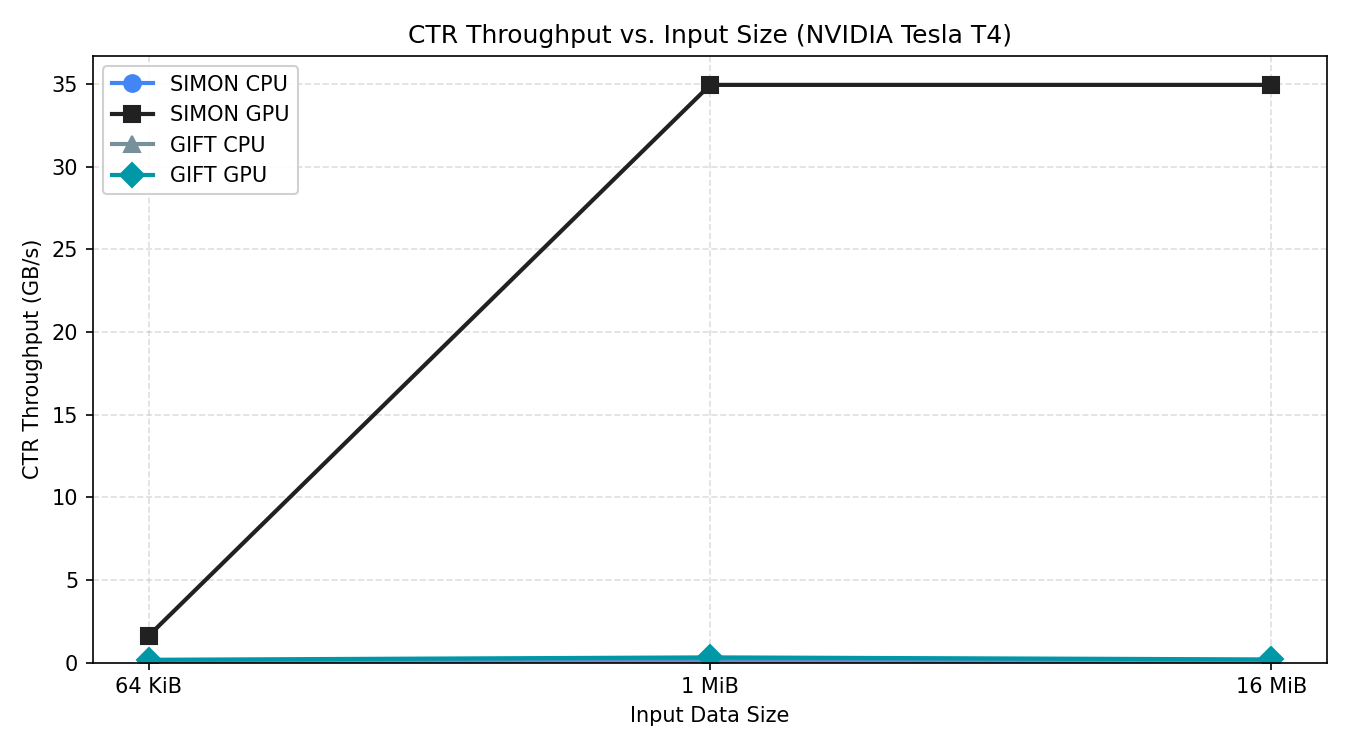
\includegraphics[width=\linewidth]{throughput_ctr_all.png}
\caption{CTR throughput (GB/s) vs.\ input size on NVIDIA Tesla~T4
(SM~7.5, \texttt{nvcc~-O2}).}
\label{fig:throughput}
\end{figure}

Since every counter block is independent, CTR mode parallelizes
trivially on a GPU.  At small sizes (64~KiB) the kernel launch overhead
dominates and the speedup is modest, but at 16~MiB SIMON hits
\textbf{420$\times$} because its round function uses so few registers
(just shifts and XORs).  GIFT peaks at \textbf{388$\times$} for 1~MiB
but falls to 266$\times$ at 16~MiB.  We believe this is because the
permutation arrays push up register usage and reduce occupancy.
CBC encryption is still sequential by nature, though CBC
\emph{decryption} could be parallelized.

\subsection{Discussion}

The numbers paint a clear picture of where each cipher fits best.
SIMON's Feistel rounds use only register-level operations, so it is
fast in software even though it needs more rounds (44 vs.\ 40).  GIFT's
bit permutations are essentially free in hardware wiring but require
explicit bit extraction and insertion in software, which explains the
339~cpb figure.  AES is still the fastest option \emph{if} the chip has
AES-NI, but without that support the MixColumns step and large S-box
tables make it both slower and bigger than either lightweight cipher.

In practice, for something like an ARM Cortex-M0 IoT node (no AES-NI,
limited flash), SIMON is the obvious pick: 11~cpb, 356~bytes of code,
38~ns key setup.  For an ASIC or RFID tag where silicon area matters
most, GIFT at $\sim$1300~GE is the better choice.

\subsection{Security Considerations}

Both ciphers use 128-bit keys.  SIMON has been analyzed extensively:
the best published differential/linear attacks get through about 26 out
of 44~rounds~\cite{beaulieu2013simon}, so there is a solid margin.
For GIFT, the best known attacks cover 23 of 40~rounds; the
non-involutory S-box was chosen specifically to resist differential
and linear cryptanalysis.

One practical bonus is that both ciphers run in constant time.  SIMON
has no lookup tables at all, and GIFT applies its S-box
nibble-by-nibble (which can be done with bitwise ops).  Neither cipher
has data-dependent memory access patterns, so they are not vulnerable
to cache-timing side-channel attacks the way table-based AES can be.

%===================================================================
\section{Conclusion}
%===================================================================

We built working C implementations of SIMON~64/128 and GIFT-128/128
with CBC and CTR modes, verified them against spec test vectors, and
benchmarked them against hardware-accelerated AES-128.  We also wrote
CUDA kernels for both ciphers and ran them on a Tesla~T4.

The takeaway is pretty clear: on platforms without AES-NI, lightweight
ciphers are worth considering.  SIMON in particular gives 11~cpb in
only 356~bytes of code, and on a GPU it scales to a 420$\times$
speedup in CTR mode.  GIFT is much slower in software but comes in
at roughly 1300~GE in hardware, which matters for RFID and similar
area-constrained designs.

From a design perspective, the Feistel vs.\ SPN choice matters a lot.
SIMON wins on every software metric we measured (CPU throughput, code
size, GPU speedup), while GIFT wins on hardware area.  For anyone
choosing a lightweight cipher, the decision should come down to
whether the implementation target is software or silicon.

%===================================================================
\section*{Acknowledgment}
%===================================================================

This work was completed as part of ECE~268 at UC San Diego, Spring~2026.

\begin{thebibliography}{00}

\bibitem{bogdanov2007present}
A.~Bogdanov, L.~R.~Knudsen, G.~Leander, C.~Paar, A.~Poschmann,
M.~J.~B.~Robshaw, Y.~Seurin, and C.~Vikkelsoe,
``PRESENT: An ultra-lightweight block cipher,''
in \emph{Proc.\ CHES 2007}, ser.\ LNCS, vol.~4727.\hskip 1em
Springer, 2007, pp.~450--466.

\bibitem{beaulieu2013simon}
R.~Beaulieu, D.~Shors, J.~Smith, S.~Treatman-Clark, B.~Weeks, and
L.~Wingers,
``The SIMON and SPECK families of lightweight block ciphers,''
IACR ePrint 2013/404, 2013.

\bibitem{banik2017gift}
S.~Banik, S.~K.~Pandey, T.~Peyrin, Y.~Sasaki, S.~M.~Sim, and Y.~Todo,
``GIFT: A small present---towards reaching the limit of lightweight
encryption,''
in \emph{Proc.\ CHES 2017}, ser.\ LNCS, vol.~10529.\hskip 1em
Springer, 2017, pp.~321--345.

\bibitem{feldhofer2004strong}
M.~Feldhofer, S.~Dominikus, and J.~Wolkerstorfer,
``Strong authentication for RFID systems using the AES algorithm,''
in \emph{Proc.\ CHES 2004}, ser.\ LNCS, vol.~3156.\hskip 1em
Springer, 2004, pp.~357--370.

\bibitem{giftref}
S.~M.~Sim, ``GIFT reference implementation,''
\url{https://github.com/giftcipher/gift}, 2017.

\end{thebibliography}

\end{document}
